\section{Piattaforma di sviluppo}
In questa sezione si descrive come è composta e come è stata assemblata la piattaforma per lo sviluppo e il testing.

\subsection{Rover AgileX}
Il veicolo selezionato per lo sviluppo della presente tesi è un rover terrestre prodotto da AgileX, modello Hunter. Questo rover è dotato di 3 motori elettrici (2 per la trazione posteriore ed 1 per lo sterzo), di sensori dediti all'analisi del movimento delle ruote e di una board utile per l'interfacciamento del mezzo con un calcolatore esterno. L'intera scocca è realizzata in alluminio rendendolo molto resistente ma allo stesso tempo non eccessivamente pesante.

\begin{figure}[h!]
  \centering
  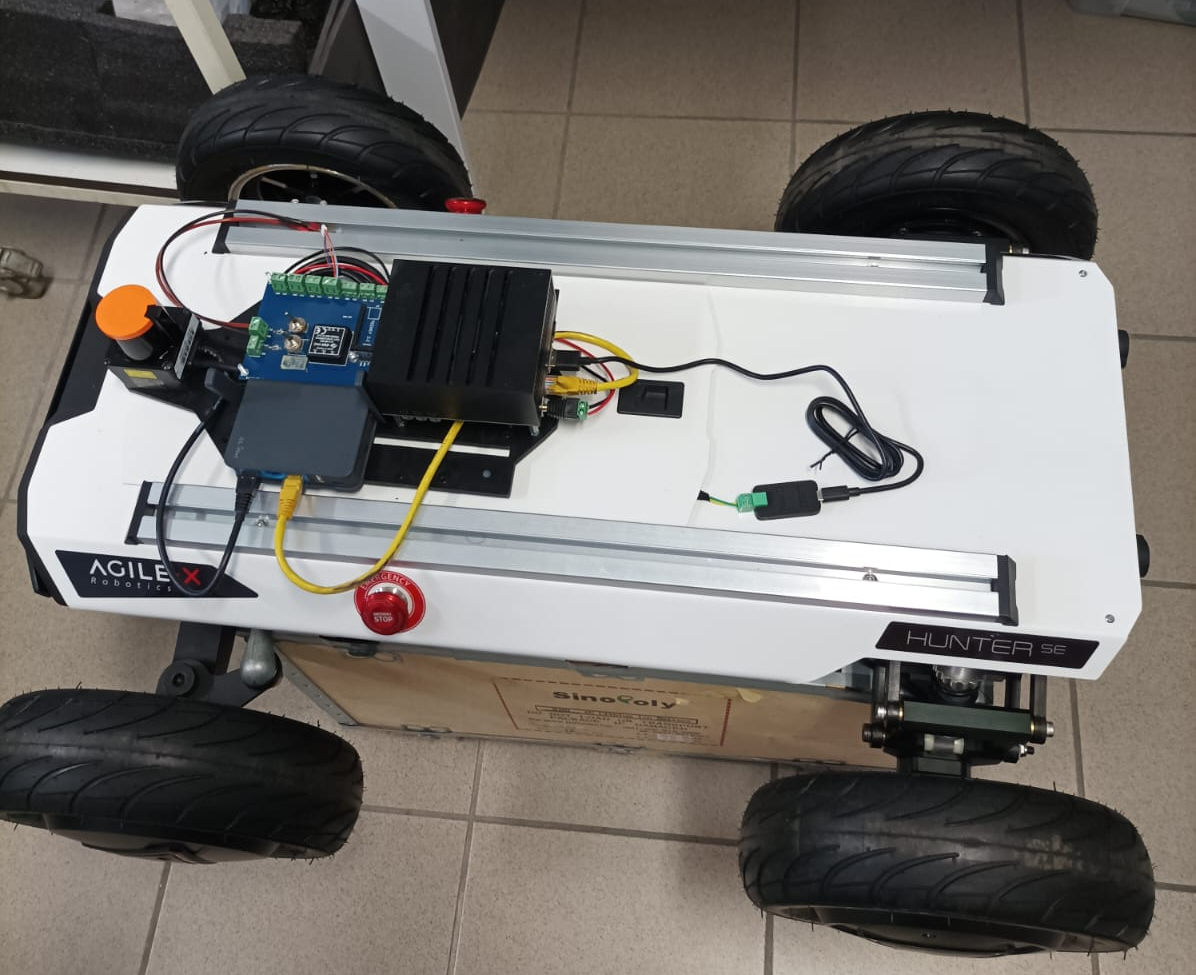
\includegraphics[width=1\textwidth]{figures/franco.png}
  \caption{Rover assemblato}
  \label{Rover assemblato}
\end{figure}

\noindent L'interfaccia di controllo del rover è collegata alla porta usb del computer embedded e consente una comunicazione efficiente e affidabile con esso. Il modello Hunter è stato scelto per le sue avanzate caratteristiche tecniche e per la sua versatilità, che lo rendono particolarmente adatto alle esigenze del progetto.

\noindent Oltre a fornire un'interfaccia per il controllo diretto, il veicolo è in grado di raccogliere e trasmettere una serie di dati diagnostici e operativi fondamentali per il monitoraggio e l'analisi delle sue prestazioni. Tra questi dati, un ruolo cruciale è ricoperto dall'odometria. 

\noindent L'odometria è una misura che permettte la stima dello spostamento di un veicolo su ruote a partire dallo spostamento di esse, questa è essenziale per la navigazione e la stima della posizione del rover, poiché permette di determinare il percorso seguito dal veicolo e la distanza percorsa. Questi dati, insieme ad altre informazioni sullo stato del veicolo, contribuiscono a garantire un controllo preciso e ad alimentare i sistemi di guida autonoma e remota previsti dal progetto.

\subsubsection{Protocollo CAN}
L'interfaccia di controllo del rover è basata sul protocollo CAN (Controller Area Network), un protocollo seriale molto versatile sviluppato dall'azienda Bosh nel 1993 ed è molto utilizzato in ambito automotive e automazione industriale. Questa interfaccia seriale è accessibile tramite 2 cavi denominati HIGH e LOW, collegati ad un interfaccia USB a cui poi il computer di bordo si va a interfacciare.

Il protocollo CAN è utilizzato in quanto è un protocollo molto resistente alle interferenze (grazie a una tecnica di bit dominante e recessivo), veloce e per niente costoso.  

\subsection{GPGPU}
Un elemento cruciale per la realizzazione di questa tesi è stato l'identificazione e la selezione di un calcolatore embedded che possa prima di tutto comunicare con i sensori e il rover ed inoltre che possa anche gestire il carico di tutti gli algoritmi e i processi necessari per la guida autonoma.

\noindent La scelta è dunque ricaduta su una scheda di casa Nvidia, nello specifico sul modello AGX Jetson Xavier, ovvero una GPGPU (General Purpose Graphic Processing Unit). Questa scelta è motivata dall'elevata capacità di elaborazione parallela che solo una GPGPU può fornire, questa capacità risulta particolarmente vantaggiosa per l'esecuzione di complessi algoritmi di percezione e pianificazione, oltre che di controllo, da svolgere in tempo reale. La GPGPU selezionata opera con il sistema operativo Ubuntu 20.04 Focal Fossa, noto per la sua stabilità e ampia compatibilità con l'hardware scelto.

\subsection{Lidar}
Per quanto concerne il sensore, la scelta è ricaduta su un sensore Lidar (Light Detection and Ranging) a 2 dimensioni. Questo dispositivo sfrutta la tecnologia laser per determinare la distanza di vari punti nell'ambiente circostante, calcolando il tempo di ritorno dei raggi laser emessi. Il Lidar fornisce una mappa dettagliata della topografia dell'ambiente, consentendo al sistema di percezione di creare rappresentazioni, tridimensionali o bidimensionali a seconda della tipologia, accurate e fondamentali per il riconoscimento degli ostacoli, la navigazione, la pianificazione del percorso del veicolo e la mappatura dell'ambiente circostante. La combinazione di una GPGPU performante e un sensore Lidar avanzato rappresenta una solida base tecnologica per lo sviluppo di un sistema di guida autonoma e remota altamente efficiente.

\noindent Il sensore Lidar genera una nuvola di punti dell'ambiente circostante attraverso l'emissione di impulsi laser in un cono di 270 gradi. Ciascun punto della nuvola corrisponde alla distanza misurata tra il sensore e un elemento dell'ambiente. La distanza è determinata con accuratezza cronometrando il tempo impiegato dall'impulso laser a percorrere il tragitto andata e ritorno.

\noindent Di seguito un'immagine che dimostra intuitavemente il funzionamento del sensore Lidar.

\begin{figure}[h!]
  \centering
  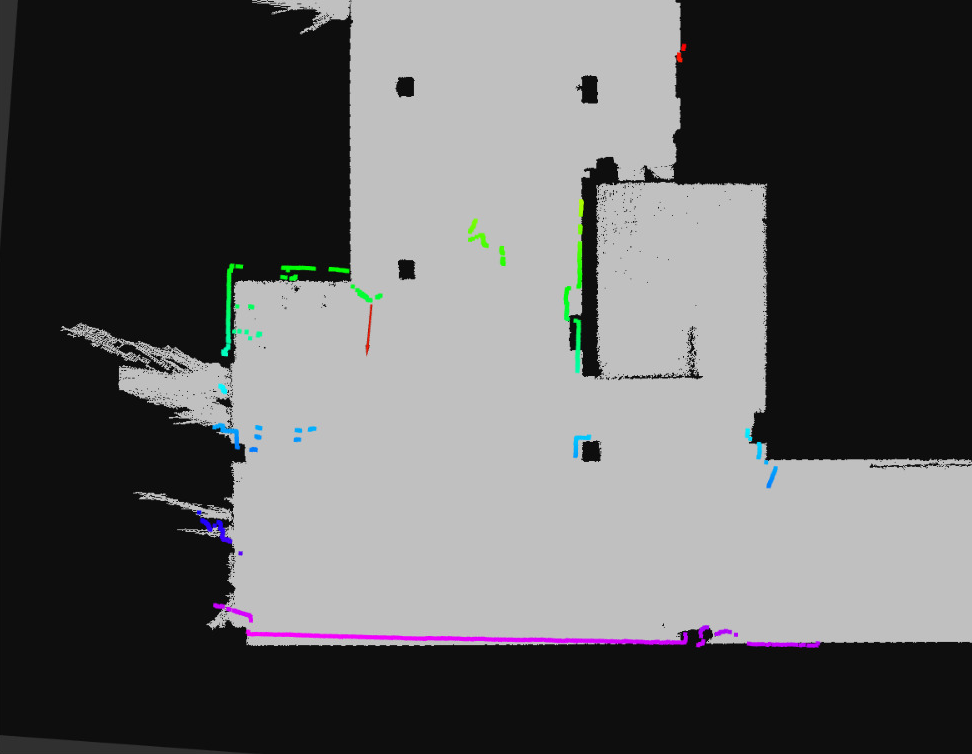
\includegraphics[width=1\textwidth]{figures/lidar_map.png}
  \caption{Dimostrazione funzionamento del sensore Lidar}
  \label{Dimostrazione funzionamento del sensore Lidar}
\end{figure}

\noindent In questa immagine abbiamo una porzione di una mappa(lo sfondo nero e grigio) e la pointcloud generata dal sensore Lidar (i punti colorati). Il colore dei punti non è casuale, bensì il colore è un metodo intuitivo per stimare la distanza di quel particolare punto dal robot (la freccia rossa).

\subsection{Router}
In considerazione delle elevate esigenze di comunicazione proprie di un veicolo connesso, si è optato per l'integrazione a bordo di un router di rete. Tale dispositivo ha la duplice funzione di stabilire una connessione stabile e ad alta banda passante con l'infrastruttura di rete esterna, garantendo così la trasmissione fluida dei dati, e di fungere da nodo centrale per la comunicazione interna al veicolo. In particolare, il router è preposto a interconnettere il calcolatore di bordo, deputato all'elaborazione dei dati provenienti dai vari sensori, con il sensore Lidar, il quale, mediante interfaccia Ethernet, trasmette ingenti volumi di dati destinati al calcolatore.

